\chapter{Comparative Genomic Analysis of \emph{P. papatasi} and \emph{L. longipalpis} Sand Fly Genomes}

\section{Introduction}

\section{Methods}

\subsection{Data sets}


The \emph{Ae. aegypti}, \emph{An. gambiae}, \emph{L. longipalpis}, and \emph{P. papatasi} \textcolor{red}{TODO VERSIONS} peptide translations were downloaded from Vectorbase \textcolor{red}{TODO CITE}, while the \emph{D. melanogaster} and \emph{D. simulans} peptide translations were downloaded from Flybase \textcolor{red}{TODO CITE}.

\textcolor{red}{table of versions}


\subsection{Calculation of Scaffold Gene CDF}
The gene counts of each genome's scaffolds were normalized by dividing the gene counts by the number of genes in that organism's genome. For each genome, lists of the normalized gene counts were sorted largest to smallest and padded with 0-value entries so that all of the lists had the same length.  Cumulative sums were computed over the normalized gene counts and plotted.


\subsection{Generation of Dot Plots for Macrosynteny} \label{sec:synteny-methods-dotplots}
The identifiers, scaffolds, locations, and sense in the FASTA headers were extracted for each peptide sequence.  The protein IDs were cross-referenced with OrthoDB to group the proteins into ortholog groups.  Sequences without ortholog information or no orthologs in the other genomes and ortholog groups with many-to-many and one-to-many relationships were discarded.  The proteins were sorted along each scaffold by their starting coordinates, while scaffolds were ordered arbitrarily.  Scatter plots were generated by drawing dots at the positions of orthologous proteins.

\subsection{Microsynteny} \label{sec:synteny-methods-synchro}
For each genome, the identifiers, protein sequences, orientations, scaffolds, and locations extracted from FASTA files for each genome and reformatted as input for the programs CHROnicle and SynChro \textcolor{red}{TODO CITE}.  SynChro ($\Delta=5$) was run on the pairs \emph{D. melanogaster} and \emph{D. simulans}, \emph{An. gambiae} and \emph{L. longipalpis}, \emph{An. gambiae} and \emph{Ae. aegypti}, and \emph{L. longipalpis} and \emph{P. papatasi}.  Synteny blocks were extracted from the \texttt{OrthBlocks synt} files.  Three-way synteny blocks for \emph{An. gambiae}, \emph{L. longipalpis}, and \emph{P. papatasi} were constructed by finding all pairs of synteny blocks for \emph{An. gambiae} and \emph{L. longipalpis} and \emph{L. longipalpis} and \emph{P. papatasi} that overlapped by at least one gene.  

The CDF for the distribution of synteny block gene counts for each pair of organisms was computed as follows: The gene counts for each synteny block were normalized by dividing the gene counts by the total number of genes found in synteny blocks. Lists of the normalized gene counts were sorted largest to smallest.  Cumulative sums were computed over the normalized gene counts. The synteny block indices were normalized by the total number of synteny blocks.

\textcolor{red}{TODO annotation of synteny blocks, distribution plots}

\subsection{Calculation of dN/dS}

Selective constraints on gene sequence evolution were estimated using the dN/dS statistic calculated for orthologous group multiple sequence alignments. 
Protein sequences were organized into ortholog groups according to OrthoDB v8 \textcolor{red}{TODO CITE}. Groups that did not have at least one sequence from each species were discarded.  For groups with 1-to-many and many-to-many orthologs, one protein sequence was chosen randomly with uniform weights from each species. Protein multiple sequence alignments were generated using Clustal Omega \textcolor{red}{TODO CITE} and used to inform CDS alignments with the codon-aware PAL2NAL alignment program \textcolor{red}{TODO CITE}.  The yn00 program from PAML v4.8 \textcolor{red}{TODO CITE} was used to calculate dN/dS ratios for each pairs of sequences in the aligned ortholog groups.

\subsection{GO Term Distributions}

\textcolor{red}{TODO Cuffdiff}

Gene identifiers for genes marked as statistically significant by \texttt{CuffDiff} were extracted for each time point and feeding condition.  The corresponding protein sequences for each gene were extracted from the genomes.  The protein sequences were merged and run through \texttt{BLAST2GO}. \textcolor{red}{TODO CITE, VERSION}

\section{Results}

\subsection{Analysis of Genome Assembly Fragmentation}
Fragmentation of a genome assembly significantly effects comparative genomic analysis.  In particular, if the assembly produces a large number of scaffolds with only or two genes that cannot be mapped back to chromosomes, analyses such as synteny will not produce interpretable results.  To place our analyses discussed below in context, we analyzed the amount of fragmentation occurring in the sand fly genomes.  We our analysis found evidence of significant fragmentation.

\textcolor{red}{why the choices of species?}

We analyzed and compared the distribution of genes across the scaffolds from the genomes of the sand flies \emph{Ph. papatasi} and \emph{Lu. longipalpis}, mosquitoes \emph{Ae. aegypti} and \emph{An. gambiae}, and fruit flies \emph{Dr. melonagaster} and \emph{Dr. simulans} (Figure~\ref{fig:scaffolds}).  The six organisms have between 10,100 and 17,294 genes.  Assemblies of the \emph{An. gambiae} and \emph{Dr. melonagaster} genomes are relatively complete and are used as our standard for comparison.  \emph{An. gambiae} and \emph{Dr. melonagaster} both have one scaffold per chromosome with between 1,000 and 4,000 genes located on the five largest scaffolds.

The assembly of the \emph{Dr. simulans} genome is partially fragmented but still relatively complete.  The assembly has more scaffolds (1,131) than chromosomes, but sizes (in terms of genes) of the five largest scaffolds are comparable to \emph{An. gambiae} and \emph{Dr. melonagaster}.  Comparison of the cumulative distribution of gene locations from largest to smallest scaffolds suggests that a majority of \emph{Dr. simulans}'s genes are located on a small number of large scaffolds with about 10\% of the genes distributed across a number of small scaffolds.

Analysis of \emph{Ph. papatasi}, \emph{Lu. longipalpis}, and \emph{Ae. aegypti} suggest a different story, with high levels of fragmentation.  \emph{Ph. papatasi} has more than 4,300 scaffolds.  Fewer than 100 genes are located on each of the top five largest scaffolds of all three organisms.  The cumulative distribution of genes indicates that the genes of \emph{Ph. papatasi} are nearly uniformly distributed across the scaffolds.  while the genes of \emph{Lu. longipalpis} and \emph{Ae. aegypti} are mostly concentrated among a smaller number of scaffolds, more than 10\% of the genes appear to be distributed across a large number of small scaffolds.

\begin{figure}[H]
  \centering
  \begin{subfigure}[b]{0.45\textwidth}
    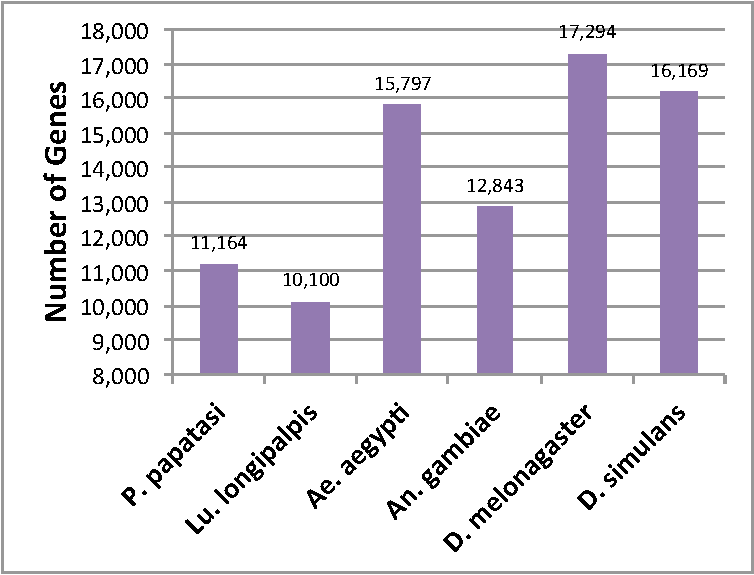
\includegraphics[width=\textwidth]{figures/synteny/genome_size_genes.pdf}
    \caption{Genome Sizes (Genes)}
  \end{subfigure}
  ~
  \begin{subfigure}[b]{0.45\textwidth}
    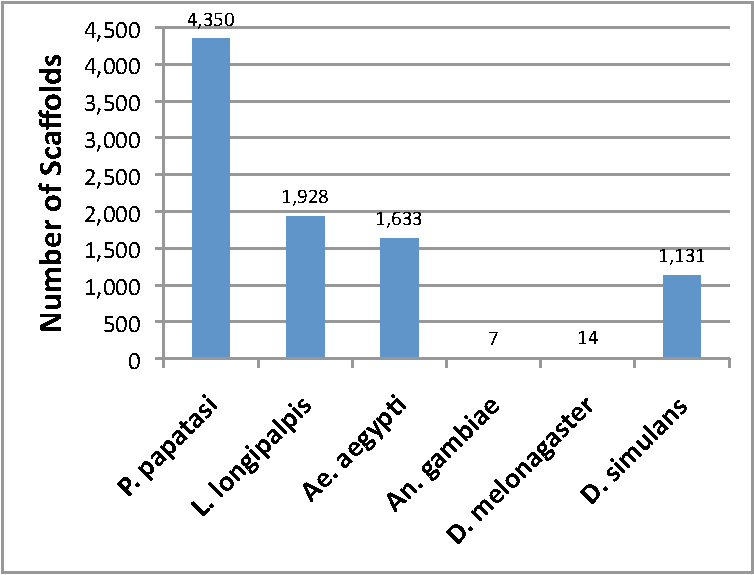
\includegraphics[width=\textwidth]{figures/synteny/scaffold_counts.pdf}
    \caption{Number of Scaffolds}
    \label{fig:number-scaffolds}
  \end{subfigure}
  ~
  \begin{subfigure}[b]{0.45\textwidth}
    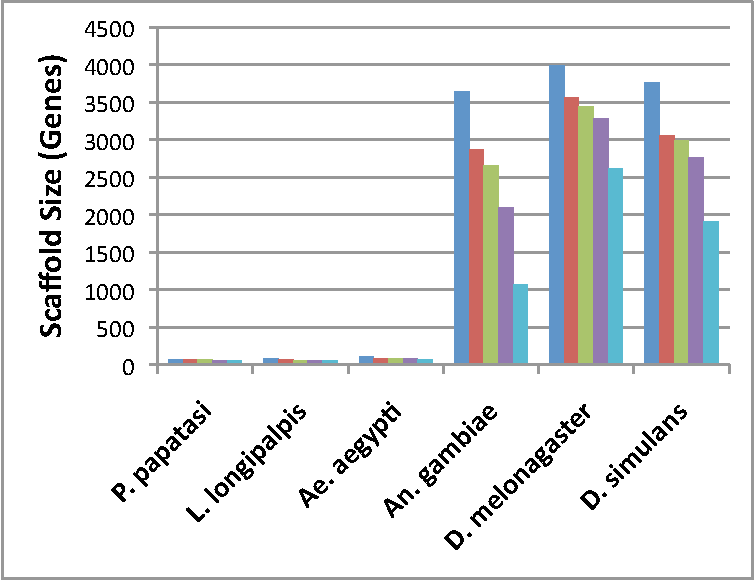
\includegraphics[width=\textwidth]{figures/synteny/top5_scaffold_sizes.pdf}
    \caption{Top 5 Scaffold Sizes (Genes)}
  \end{subfigure}
  ~
  \begin{subfigure}[b]{0.45\textwidth}
    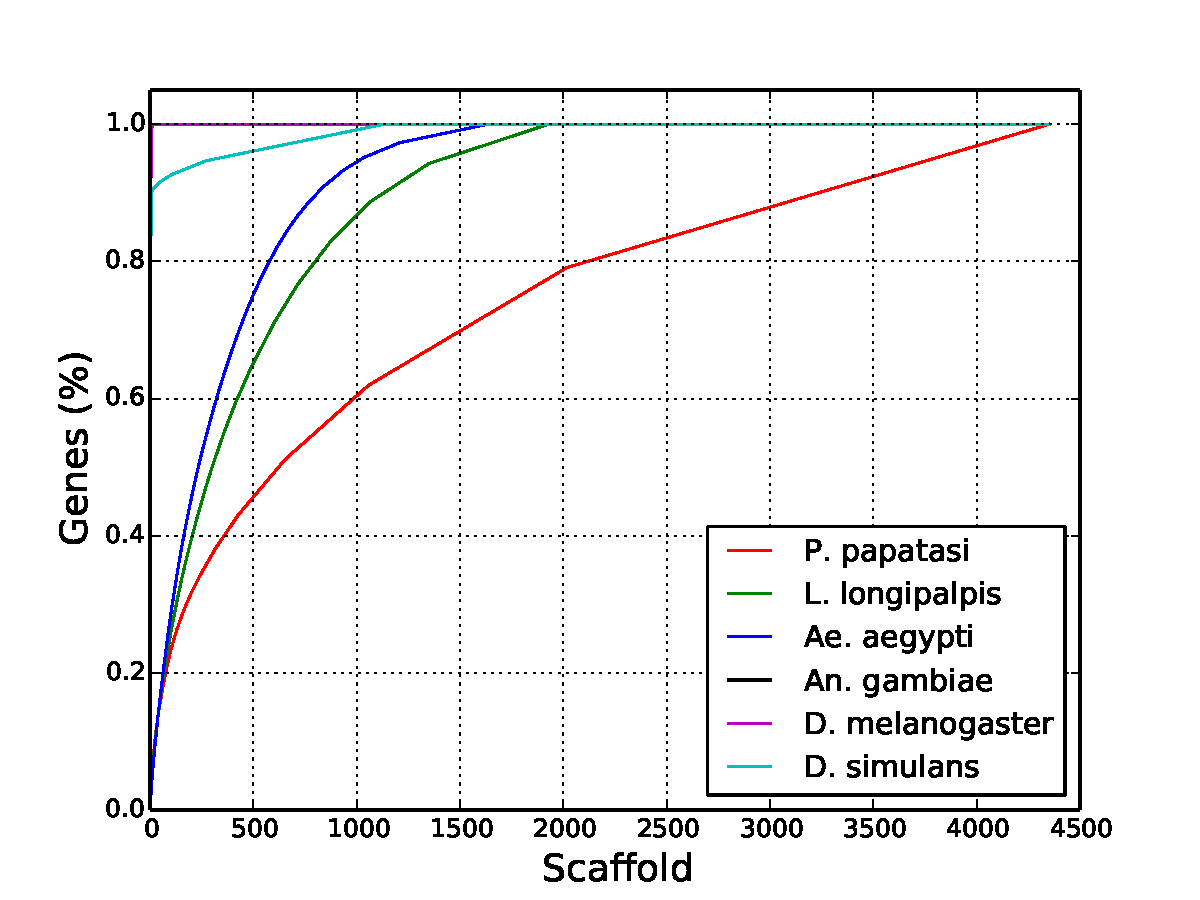
\includegraphics[width=\textwidth]{figures/synteny/gene_scaffold_cdf.pdf}
    \caption{Scaffold Genes CDF}
  \end{subfigure}
  \label{fig:scaffolds}
  \caption{}
\end{figure}

\subsection{Qualitative Analysis of Synteny}
Rearrangements of chromosomes are rare events and tend to happen in a block-wise fashion that mainly preserves the local order of genes on the chromosome. Thus, even after long periods of divergence between species, synteny blocks, defined as conserved runs of consecutive orthologous genes, remain discernible. \textcolor{red}{CITE Heger}.  The presence of synteny can be used to infer evolutionary relationships between organisms at a macroscopic level, complementing analyses such as gene family expansions and reductions and changes within pairs of orthologous genes \textcolor{red}{CITE Zdobnov}.

Synteny between pairs of dipterans was analyzed qualitatively by generating scatter plots where each axis represents genes locations for one species and dots are drawn where orthologs occur (see Section~\ref{sec:synteny-methods-dotplots}). The presence of synteny was not detectable in a qualitative comparison of \emph{L. longipalpis} and \emph{P. papatasi} (Figure~\ref{fig:synteny-dotplots-sandflies}).  In contrast, there was extensive qualitative evidence of synteny between \emph{D. melanogaster} and \emph{D. simulans} (Figure~\ref{fig:synteny-dotplots-drosophila}).  Qualitative comparison of \emph{A. gambiae} and \emph{D. melanogaster} indicated the co-location of orthologous genes on the same chromosomes but not synteny (Figure~\ref{fig:synteny-dotplots-anopheles-drosophila}). \textcolor{red}{TODO CITE co-location}

\textcolor{red}{compare Anopheles vs Dmel to Zdobnov paper}

\textcolor{red}{how long ago have the genomes diverged?}

\textcolor{red}{TODO CITE synteny of insects}

\textcolor{red}{comparison of sand flies to mosquitoes and drosophila}

\begin{figure}[H]
  \centering
  \begin{subfigure}[b]{0.45\textwidth}
    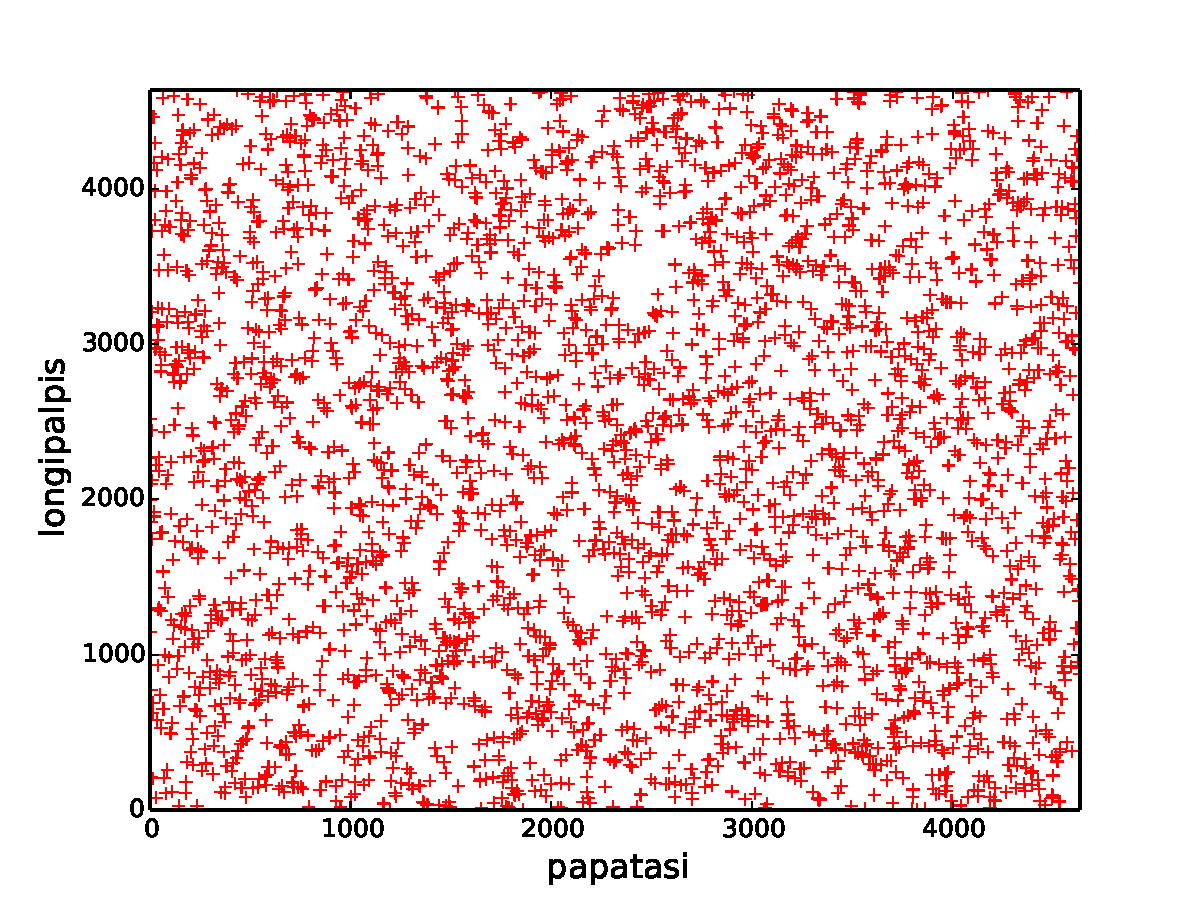
\includegraphics[width=\textwidth]{figures/synteny/papatasi_longipalpis_plot}
    \caption{\emph{L. longipalpis} vs. \emph{P. papatasi}}
    \label{fig:synteny-dotplots-sandflies}
  \end{subfigure}
  \\
  \begin{subfigure}[b]{0.45\textwidth}
    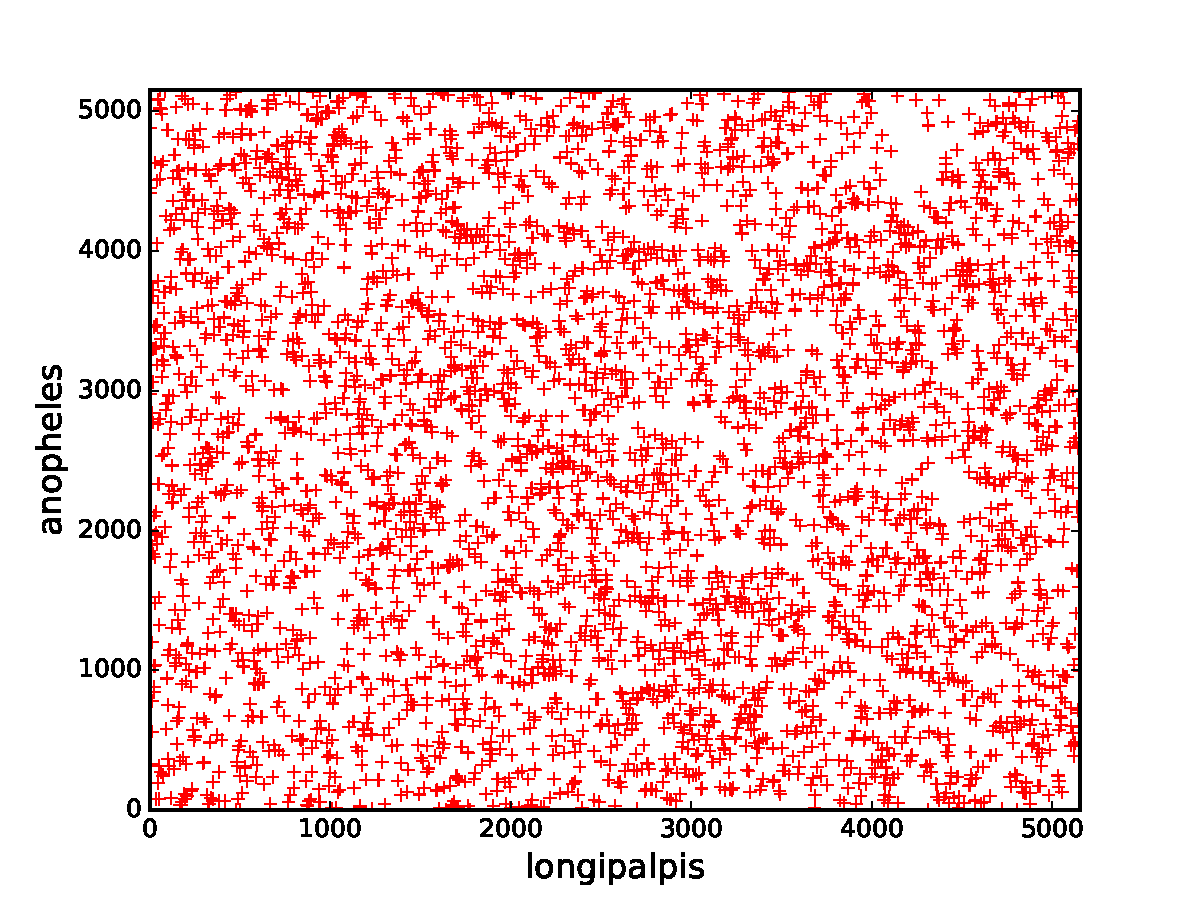
\includegraphics[width=\textwidth]{figures/synteny/longipalpis_anopheles_plot}
    \caption{\emph{L. longipalpis} vs. \emph{An. gambiae}}
    \label{fig:synteny-dotplots-longipalpis-anopheles}
  \end{subfigure}
  ~
  \begin{subfigure}[b]{0.45\textwidth}
    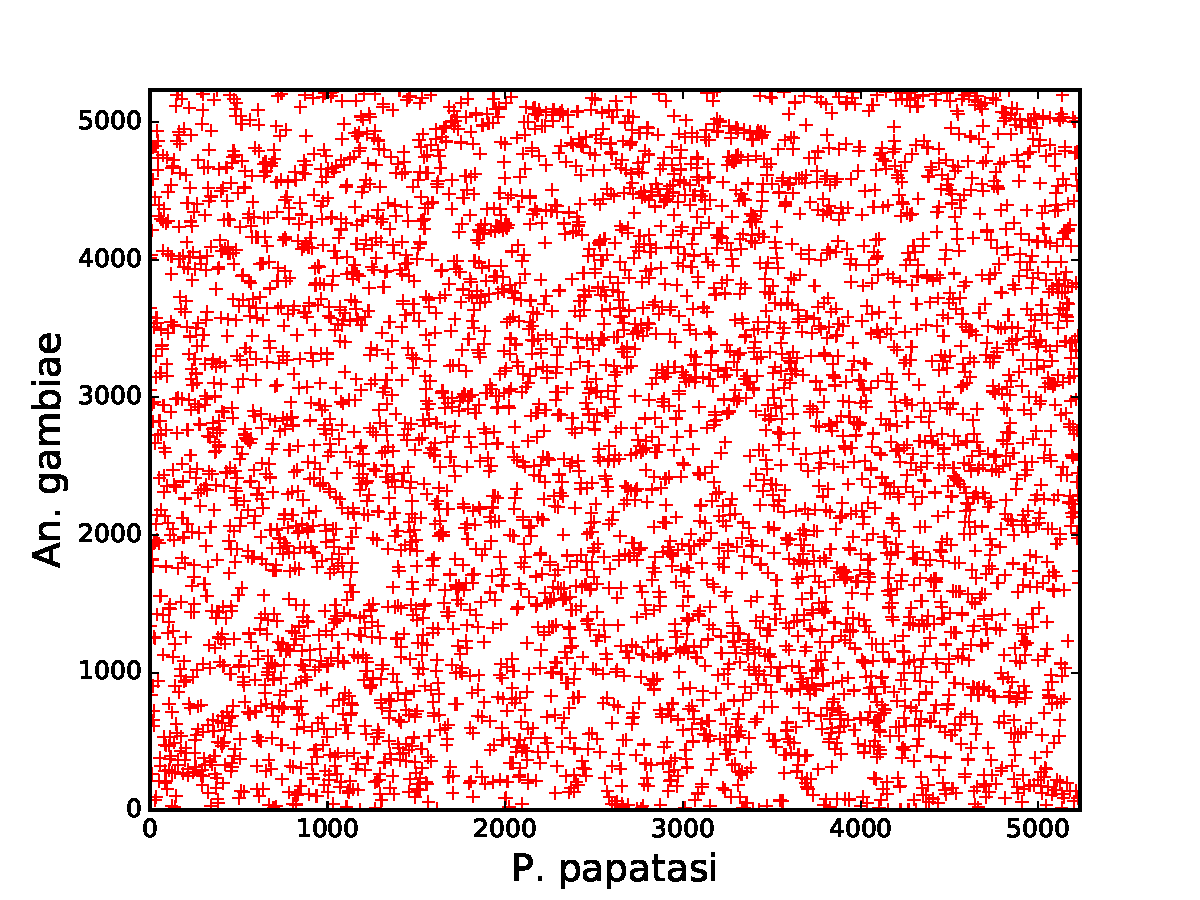
\includegraphics[width=\textwidth]{figures/synteny/papatasi_anopheles_plot}
    \caption{\emph{P. papatasi} vs. \emph{An. gambiae}}
    \label{fig:synteny-dotplots-papatasi-anopheles}
  \end{subfigure}
  ~
  \begin{subfigure}[b]{0.45\textwidth}
    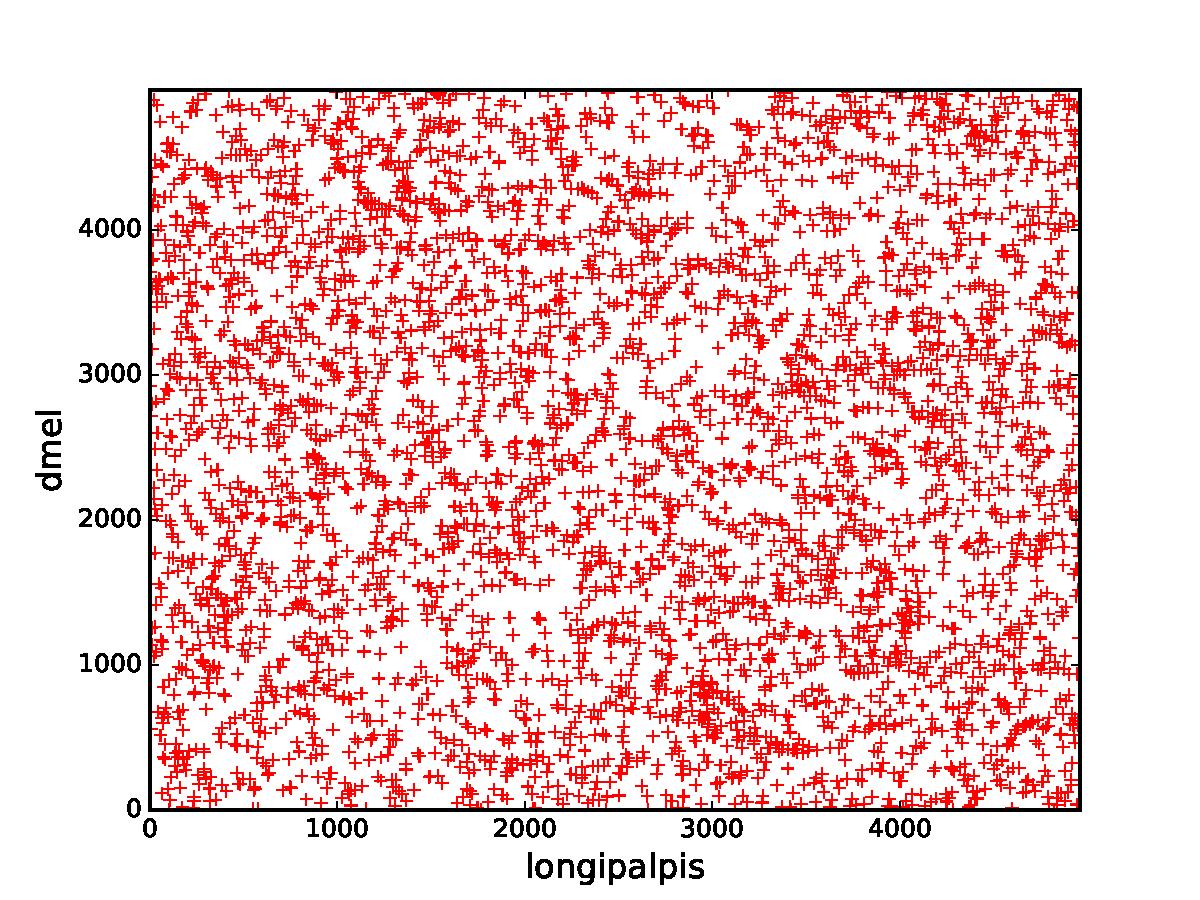
\includegraphics[width=\textwidth]{figures/synteny/longipalpis_dmel_plot}
    \caption{\emph{L. longipalpis} vs. \emph{D. melanogaster}}
    \label{fig:synteny-dotplots-longipalpis-dmel}
  \end{subfigure}
  ~
  \begin{subfigure}[b]{0.45\textwidth}
    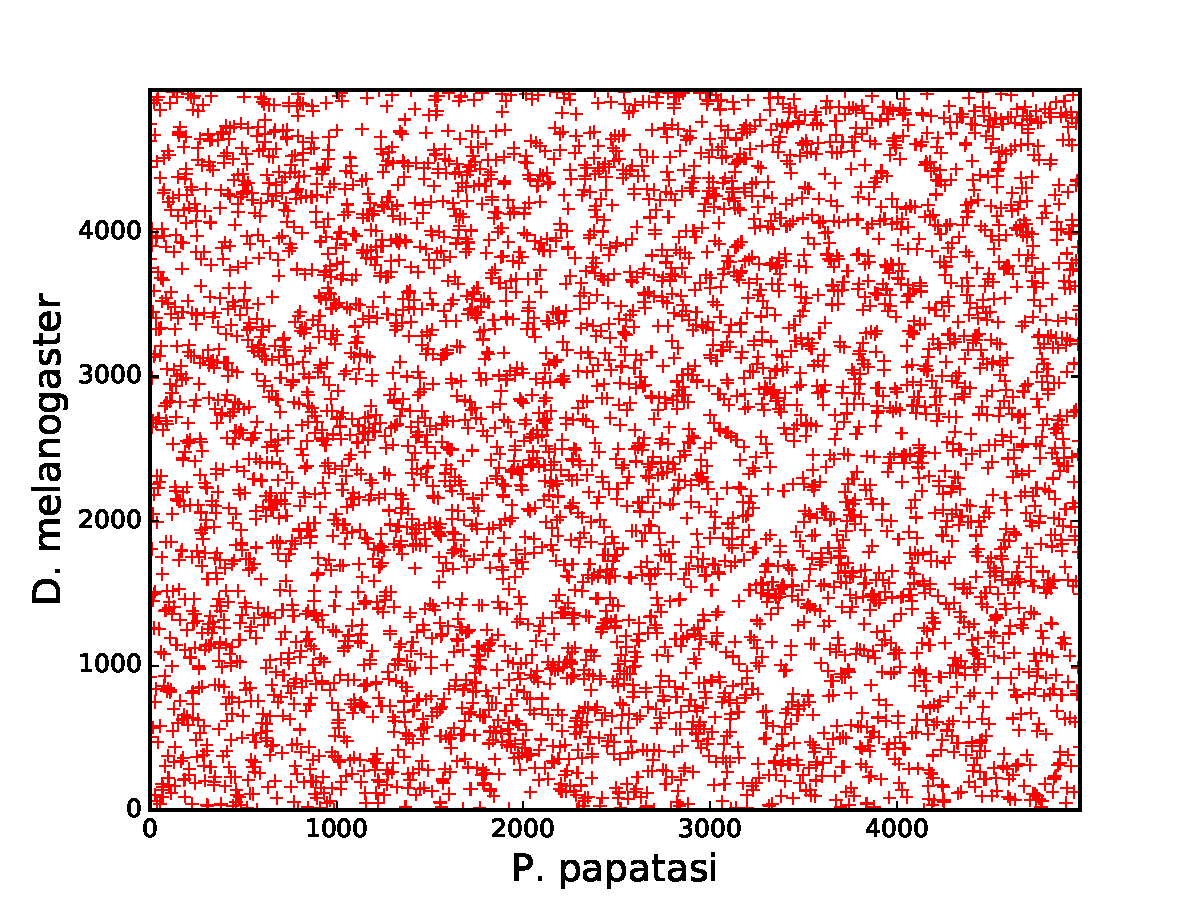
\includegraphics[width=\textwidth]{figures/synteny/papatasi_dmel_plot}
    \caption{\emph{P. papatasi} vs. \emph{D. melanogaster}}
    \label{fig:synteny-dotplots-papatasi-dmel}
  \end{subfigure}
  ~
  \begin{subfigure}[b]{0.45\textwidth}
    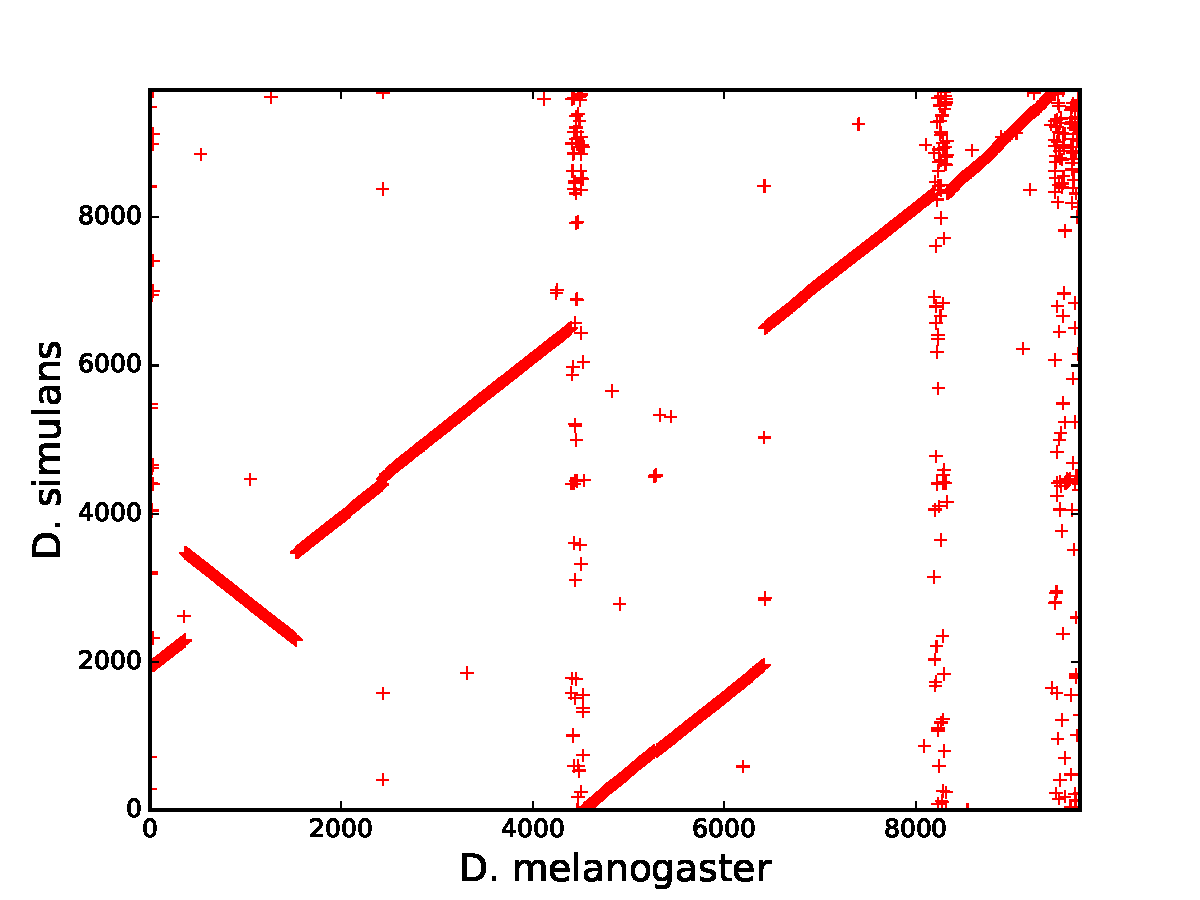
\includegraphics[width=\textwidth]{figures/synteny/dmel_dsim_plot}
    \caption{\emph{D. melanogaster} vs. \emph{D. simulans}}
    \label{fig:synteny-dotplots-drosophila}
  \end{subfigure}
  ~
  \begin{subfigure}[b]{0.45\textwidth}
    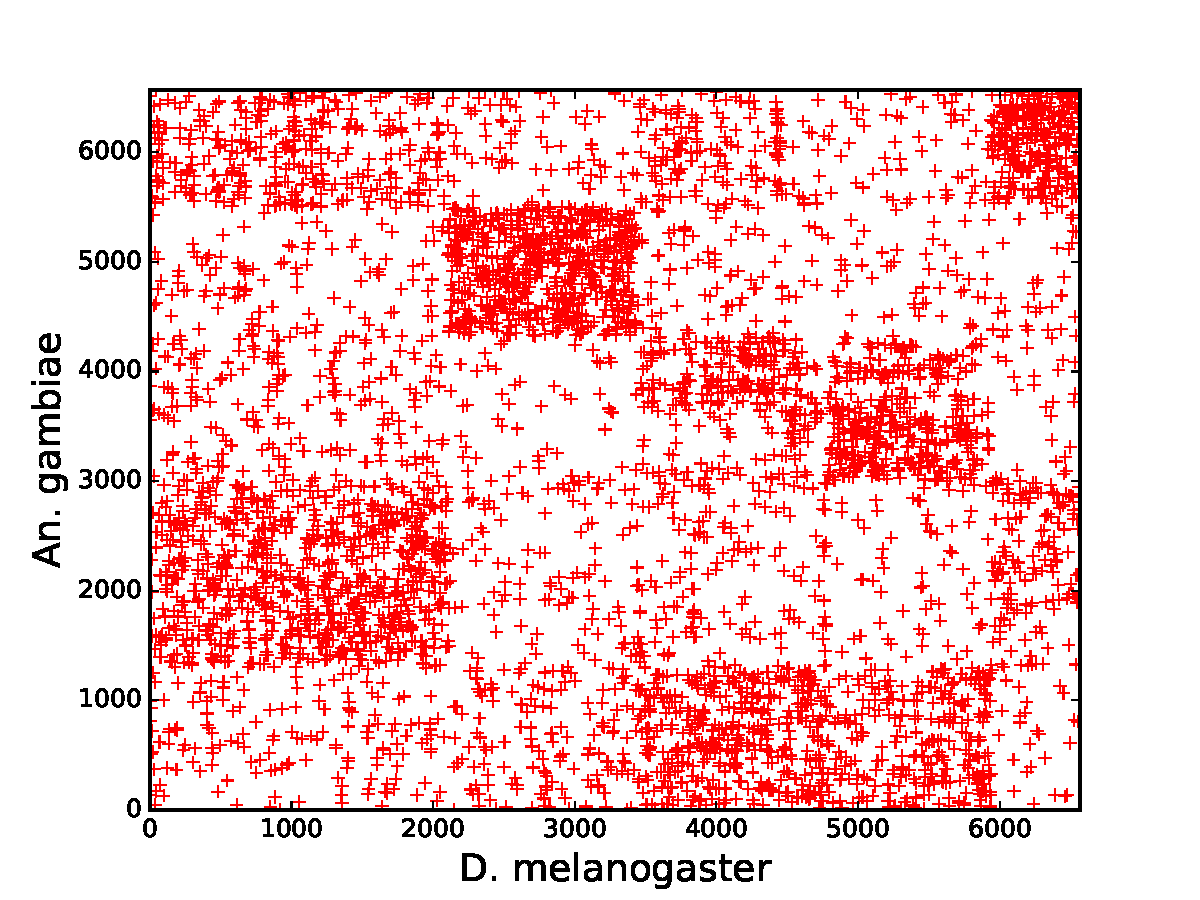
\includegraphics[width=\textwidth]{figures/synteny/dmel_anopheles_plot}
    \caption{\emph{A. gambiae} vs. \emph{D. melanogaster}}
    \label{fig:synteny-dotplots-anopheles-drosophila}
  \end{subfigure}
\label{fig:dot-plots}
\caption{Qualitative Analysis of Synteny}
\end{figure}

\begin{table}[H]
  \centering
  \begin{tabular}{c c c c c} \hline
    \emph{Species} & \emph{Count} & \emph{Average Size} & \emph{Median Size} & {Maximum Size} \\ \hline
    \emph{L. longipalpis} vs. \emph{An. gambiae} & 504 & 4.3 & 3 & 39 \\
    \emph{L. longipalpis} vs. \emph{P. papatasi} & 499 & 4.2 & 3 & 24 \\
    \emph{P. papatasi} vs. \emph{An. gambiae} & 307 & 4.3 & 3 & 21 \\
    \emph{D. melanogaster} vs. \emph{D. simulans} & 243 & 41.6 & 5 & 700 \\
    \emph{D. melanogaster} vs. \emph{An. gambiae} & 1037 & 2.5 & 2 & 10
  \end{tabular}
  \caption{Statistics including count and size (gene count) distributions for synteny blocks.}
  \label{tab:synteny-block-stats}
\end{table}

We followed up the qualitative analysis up with a quantitative analysis of synteny blocks. Synteny blocks were found between pairs of dipterans using the program SynChro (see Section~\ref{sec:synteny-methods-synchro}). As indicated by the qualitative analysis, synteny was most conserved between \emph{D. melanogaster} and \emph{D. simulans} (243 synteny blocks with the largest block size of 700 genes, an average size of 41.6 genes, and a median size of 5 genes).  When compared to each other or \emph{An. gambiae}, the sand flies exhibited little conservation of synteny with the largest blocks consisting of far fewer genes than those from \emph{D. melanogaster} and \emph{D. simulans} (24 genes from \emph{L. longipalpis} and \emph{P. papatasi}, 39 genes from \emph{L. longipalpis} vs. \emph{An. gambiae}, and 21 genes from \emph{P. papatasi} vs. \emph{An. gambiae}).

We annotated and analyzed the largest synteny blocks from \emph{L. longipalpis} and \emph{P. papatasi}. and a three-way comparison of \emph{An. gambiae}, \emph{L. longipalpis}, and \emph{P. papatasi}.  Four of the largest synteny blocks from \emph{L. longipalpis} and \emph{P. papatasi} contained genes associated with peritrophic matrices (see Table~\ref{tab:synteny-llot-ppat-peritrophic}), membrane-bound or -associated genes (see Table~\ref{tab:synteny-llot-ppat-membrane}), RNA regulation and synthesis (see Table~\ref{tab:synteny-llot-ppat-rna}), and intracellular processes (see Table~\ref{tab:synteny-llot-ppat-intracellular}). \textcolor{red}{bookkeeping genes?}

\textcolor{red}{three-way comparison}

\begin{table}[H]
  \centering
  \begin{tabular}{c c l} \hline
    \emph{L. longipalpis} & \emph{P. papatasi} & \emph{Description} \\ \hline
    LLOTMP006493 & PPATMP009348 & SCP-related protein \\
    LLOTMP006494 & PPATMP009349 & ribosomal protein S23 \\
    LLOTMP006495 & PPATMP009350 & obstructor-like \\
    LLOTMP006496 & PPATMP009351 & obstructor-like \\
    LLOTMP006497 & PPATMP009352 & obstructor-like \\
    LLOTMP006498 & PPATMP009353 & obstructor-like \\
    LLOTMP006499 & PPATMP009355 & obstructor-like \\
    LLOTMP006500 & PPATMP009356 & obstructor-like
  \end{tabular}
  \caption{Synteny block of peritrophic matrix-associated genes from \emph{L. longipalpis} vs. \emph{P. papatasi}.}
  \label{tab:synteny-llot-ppat-peritrophic}
\end{table}

\begin{table}[H]
  \centering
  \begin{tabular}{c c l} \hline
    \emph{L. longipalpis} & \emph{P. papatasi} & \emph{Description} \\ \hline
    LLOTMP010087 & PPATMP006236 & G Protein-Coupled Receptor (GPCR) \\
    LLOTMP010088 & PPATMP006238 & LIM containing protein \\
    LLOTMP010090 & PPATMP006239 & Angiotensin-converting enzyme part of the DUF1279 Superfamily \\
    LLOTMP010089 & PPATMP006241 & mitochondrial uncoupling (transporter) protein \\
    LLOTMP010091 & PPATMP006242 & farnesoic acid O-methyltransferase \\
    LLOTMP010092 & PPATMP006243 & GPI-anchored Ly-6 like \\
    LLOTMP010093 & PPATMP006244 & GPI-anchored Ly-6 like \\
    LLOTMP010095 & PPATMP006245 & tensin (actin binding)
    \end{tabular}
    \caption{Synteny block of membrane-bound or -associated genes from \emph{L. longipalpis} vs. \emph{P. papatasi}.}
  \label{tab:synteny-llot-ppat-membrane}
\end{table}

\begin{table}[H]
  \centering
  \begin{tabular}{c c l} \hline
    \emph{L. longipalpis} & \emph{P. papatasi} & \emph{Description} \\ \hline
    LLOTMP003539 & PPATMP002224 & activin receptor \\
    LLOTMP003538 & PPATMP002225 & MED20 \\
    LLOTMP003537 & PPATMP002226 & cAMP-dependent protein kinase 3 \\
    LLOTMP003535 & PPATMP002228 & Spase 25-subunit 2 \\
    LLOTMP003534 & PPATMP002229 & Sterile20-like kinase \\
    LLOTMP003530 & PPATMP002230 & upstream of RpIII128 (GTP-binding) \\
    LLOTMP003532 & PPATMP002231 & Furin 2 \\
    LLOTMP003533 & PPATMP002232 & H/ACA ribonucleoprotein complex, subunit Gar1
    \end{tabular}
    \caption{Synteny block of genes involved in RNA regulation and synthesis from \emph{L. longipalpis} vs. \emph{P. papatasi}.}
  \label{tab:synteny-llot-ppat-rna}
\end{table}

\begin{table}[H]
  \centering
  \begin{tabular}{c c l} \hline
    \emph{L. longipalpis} & \emph{P. papatasi} & \emph{Description} \\ \hline
    LLOTMP002369 & PPATMP010432 & zinc finger containing protein \\
    LLOTMP002371 & PPATMP010432 & queuine tRNA ribosyltransferase \\
    LLOTMP002372 & PPATMP010433 & Biogenesis of lysosome-related organelles complex 1, subunit 1 \\
    LLOTMP002377 & PPATMP010437 & Ecdysone-induced protein 75B \\
    LLOTMP002378 & PPATMP010438 & AdoMet-dependent rRNA methyltransferase, Spb1 \\
    LLOTMP002383 & PPATMP010440 & Gram-negative bacteria binding protein 3 \\
    LLOTMP002384 & PPATMP010441 & forkhead domain 68A containing protein
    \end{tabular}
    \caption{Synteny block of genes involved in intracellular processes from \emph{L. longipalpis} vs. \emph{P. papatasi}.}
  \label{tab:synteny-llot-ppat-intracellular}
\end{table}

\begin{table}[H]
  \centering
  \begin{tabular}{c c c l} \hline
    \emph{L. longipalpis} & \emph{P. papatasi} & \emph{An. gambiae} & \emph{Description} \\ \hline
    LLOTMP008393 & PPATMP010957 & & Cadherin \\
    LLOTMP008394 & PPATMP010954 & AGAP009084 & PHLPP \\
    LLOTMP008396 & PPATMP010953 & AGAP009085 & cysteine-rich secretory protein 2 \\
    LLOTMP008397 & PPATMP010951 & AGAP009087 & PHLPP \\
    LLOTMP008398 & PPATMP010950 & AGAP009088 & LIM homeobox protein \\
    LLOTMP008399 & PPATMP010949 & AGAP009090 & Dopa decarboxylase \\
    LLOTMP008401 & PPATMP010948 & AGAP009091 & Dopa decarboxylase
    \end{tabular}
    \caption{Synteny block of genes involved in a dopamine signaling pathway and enzyme regulation from \emph{L. longipalpis} vs. \emph{P. papatasi} vs. \emph{An. gambiae}.}
  \label{tab:synteny-three-way-dopamine}
\end{table}

\begin{table}[H]
  \centering
  \begin{tabular}{c c c l} \hline
    \emph{L. longipalpis} & \emph{P. papatasi} & \emph{An. gambiae} & \emph{Description} \\ \hline
    LLOTMP001853 & PPATMP007803 & AGAP002847 & Niemann-Pick like \\
    LLOTMP001854 & PPATMP007804 & AGAP002848 & Niemann-Pick like \\
    LLOTMP001855 & PPATMP007805 & AGAP002849 & Niemann-Pick like \\
    LLOTMP001857 & PPATMP007806 & AGAP002850 & Niemann-Pick like \\
    LLOTMP001858 & PPATMP007807 & AGAP002851 & Niemann-Pick like \\
    LLOTMP001859 & PPATMP007808 & AGAP002852 & Niemann-Pick like \\
    LLOTMP001861 & & AGAP002853 & Niemann-Pick like \\
    LLOTMP001863 & & AGAP002854 & Niemann-Pick like \\
    LLOTMP001864 & & AGAP002855 & Niemann-Pick like \\
    LLOTMP001865 & & AGAP002857 & Niemann-Pick like
    \end{tabular}
    \caption{Synteny block of Niemann-Pick like genes from \emph{L. longipalpis} vs. \emph{P. papatasi} vs. \emph{An. gambiae}.}
  \label{tab:synteny-three-way-np2}
\end{table}

\begin{table}[H]
  \centering
  \begin{tabular}{c c c l} \hline
    \emph{L. longipalpis} & \emph{P. papatasi} & \emph{An. gambiae} & \emph{Description} \\ \hline
    LLOTMP004534 & PPATMP002862 & AGAP006946 & prefoldin subunit 4 \\
    LLOTMP004533 & PPATMP002863 & AGAP006945 & okra/SNF-2/RAD54 \\
    LLOTMP004535 & PPATMP002865 & AGAP006944 & eIF3/Int6 \\
    LLOTMP004536 & PPATMP002864 & AGAP006939 & Armitage \\
    LLOTMP004537 & PPATMP002868 & AGAP006942 & importin-beta \\
    LLOTMP004538 & PPATMP002870 & & (carboxyl)esterase
    \end{tabular}
    \caption{Synteny block of transcription-regulating or protein-modifying genes from \emph{L. longipalpis} vs. \emph{P. papatasi} vs. \emph{An. gambiae}.}
  \label{tab:synteny-three-way-transcription}
\end{table}

\begin{table}[H]
  \centering
  \begin{tabular}{c c c l} \hline
    \emph{L. longipalpis} & \emph{P. papatasi} & \emph{An. gambiae} & \emph{Description} \\ \hline
    LLOTMP001529 & PPATMP004782 & AGAP010568 & lipoyl synthase \\
    LLOTMP001530 & PPATMP004783 & AGAP010567 & slimfast (amino acid transporter) \\
    LLOTMP001531 & PPATMP004784 & AGAP010566 & ORMDL \\
    LLOTMP001532 & PPATMP004785 & AGAP010563 & amino acid transporter \\
    LLOTMP001533 & PPATMP004786 & AGAP010561 & slimfast (amino acid transporter)
    \end{tabular}
    \caption{Synteny block of amino acid transport or protein-modifying genes from \emph{L. longipalpis} vs. \emph{P. papatasi} vs. \emph{An. gambiae}.}
  \label{tab:synteny-three-way-amino}
\end{table}

\subsection{Comparison of $d_N$/$d_S$ Distributions}
\begin{figure}[H]
  \centering
  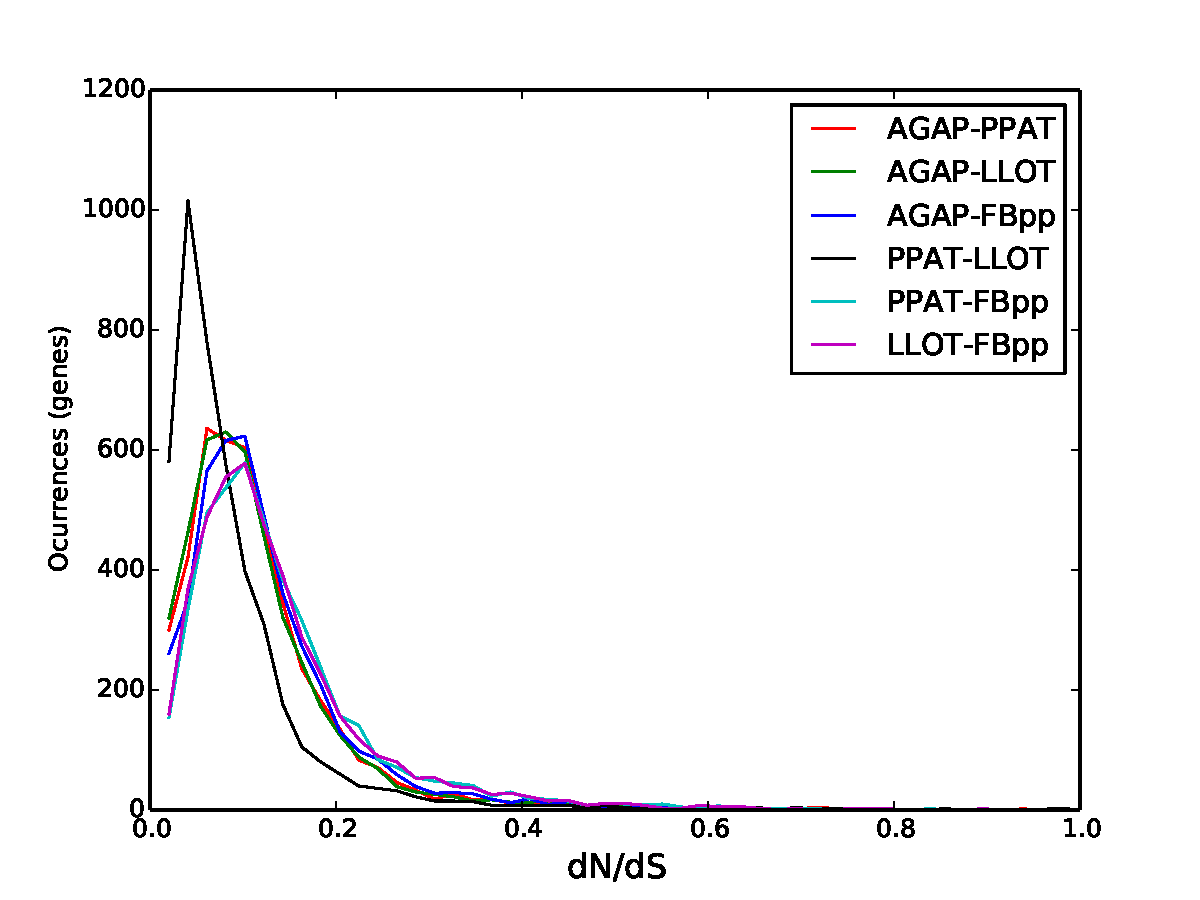
\includegraphics[width=0.75\textwidth]{figures/ka_ks/dN_dS}
  \caption{Distribution of dN/dS values}
  \label{fig:dnds-distr}
\end{figure}

\subsection{GO Term Distribution Differences}

\begin{table}[H]
  \centering
  \begin{tabular}{c c c} \hline
  \emph{Time Point} & \emph{Blood Fed vs Sugar Fed} & \emph{Infected Blood Fed vs Blood Fed} \\ \hline
  6H & 3,111 & 271 \\ \hline
  24H & 4,120 & 658 \\ \hline
  144H & 4,571 & 290 \\ \hline
  \end{tabular}
  \caption{Number of Genes with Statistically-Significant Differential Expression}
  \label{tab:stat-sig-genes}
\end{table}

\section{Discussion and Conclusion}
